\documentclass[tikz,border=8pt]{standalone}
% Shared look for every TikZ diagram. Load with \input{../../tools/tikz-style.tex}
\usepackage[sfdefault]{roboto}
\usetikzlibrary{arrows.meta, positioning, shapes.geometric, calc, fit, backgrounds}
\definecolor{cblue}{HTML}{4C78A8}
\definecolor{corange}{HTML}{F58518}
\definecolor{cgreen}{HTML}{54A24B}
\definecolor{cred}{HTML}{E45756}
\definecolor{cpurple}{HTML}{B279A2}
\definecolor{cgrey}{HTML}{6B6B6B}
\tikzset{
  every picture/.style={font=\sffamily, line width=1.2pt},
  box/.style={draw=#1, fill=#1!12, rounded corners=4pt, align=center, inner sep=7pt, minimum height=1.1cm},
  box/.default=cgrey,
  arrow/.style={-{Stealth[length=3mm]}, draw=cgrey, line width=1.4pt},
  title/.style={font=\sffamily\bfseries\Large},
  note/.style={font=\sffamily\small, text=cgrey, align=center},
}
\AtBeginDocument{\hyphenpenalty=10000 \exhyphenpenalty=10000}

% The PID loop this Note tunes, with each practical change marked by the section that adds it:
% the gains (Sections 3 and 4), the set-point weight beta and the derivative on the measurement (Section 5),
% the filter on the derivative path (Section 6). The robot is the speed loop or the heading loop.
\begin{document}
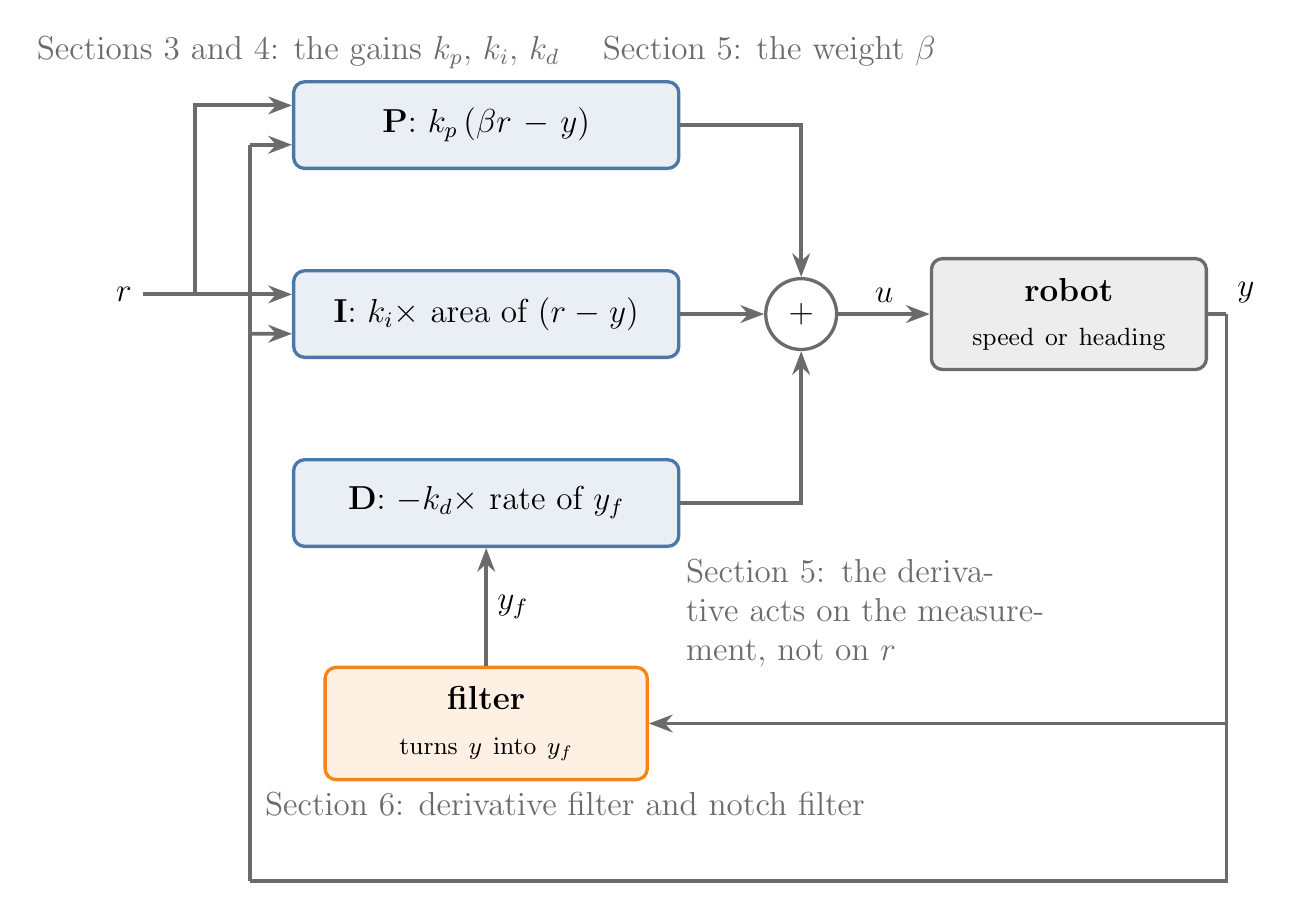
\begin{tikzpicture}[every node/.append style={font=\large}]
  \node (r) at (0,2.45) {$r$};
  \node[box=cblue, text width=4.4cm] (P) at (4.6,4.6) {\textbf{P}: $k_p\,(\beta r - y)$};
  \node[box=cblue, text width=4.4cm] (I) at (4.6,2.2) {\textbf{I}: $k_i \times$ area of $(r - y)$};
  \node[box=cblue, text width=4.4cm] (D) at (4.6,-0.2) {\textbf{D}: $-k_d \times$ rate of $y_f$};
  \node[circle, draw=cgrey, fill=white, minimum size=0.9cm, inner sep=0pt] (sum) at (8.6,2.2) {$+$};
  \node[box=cgrey, text width=3.0cm] (robot) at (12.0,2.2) {\textbf{robot}\\[2pt]\small speed or heading};
  \node[box=corange, text width=3.6cm] (filt) at (4.6,-3.0) {\textbf{filter}\\[2pt]\small turns $y$ into $y_f$};
  % reference into P and I (upper half of each box), measurement into P and I (lower half)
  \draw[arrow] (r) -- ($(I.west)+(0,0.25)$);
  \draw[arrow] (0.9,2.45) |- ($(P.west)+(0,0.25)$);
  \draw[arrow] (P.east) -| (sum.north);
  \draw[arrow] (I.east) -- (sum.west);
  \draw[arrow] (D.east) -| (sum.south);
  \draw[arrow] (sum.east) -- node[above] {$u$} (robot.west);
  \draw[draw=cgrey] (robot.east) -- (14.0,2.2) node[above right] {$y$};
  \draw[draw=cgrey] (14.0,2.2) -- (14.0,-5.0) -- (1.6,-5.0);
  \draw[arrow] (14.0,-3.0) -- (filt.east);
  \draw[draw=cgrey] (1.6,-5.0) -- (1.6,4.35);
  \draw[arrow] (1.6,4.35) -- ($(P.west)+(0,-0.25)$);
  \draw[arrow] (1.6,1.95) -- ($(I.west)+(0,-0.25)$);
  \draw[arrow] (filt.north) -- node[right] {$y_f$} (D.south);
  % where each section acts
  \node[note, font=\large, anchor=south] at (P.north) {Sections 3 and 4: the gains $k_p$, $k_i$, $k_d$ \quad Section 5: the weight $\beta$};
  \node[note, font=\large, anchor=west, text width=4.6cm, align=left] at (7.0,-1.6) {Section 5: the derivative acts on the measurement, not on $r$};
  \node[note, font=\large, anchor=north] at ($(filt.south)+(1.0,0)$) {Section 6: derivative filter and notch filter};
\end{tikzpicture}
\end{document}
